\documentclass{article}
\usepackage[utf8]{inputenc}
\usepackage[spanish]{babel}
\usepackage{natbib}
\usepackage{graphicx}
\usepackage{mathtools}
\usepackage{color}
\usepackage{float}
\usepackage{fancyhdr}
\usepackage{adjustbox}
\usepackage{verbatim}


\pagestyle{fancy}
\lhead{Grupo 4 - Turno 7}
\chead{Trabajo Practico Nro 4}
\rhead{Primer Cuatrimestre 2015}

\begin{document}
\subsection{Objetivos}
En general, el objetivo del trabajo es realizar diversas experiencias y observar cómo se producen en la realidad aquellos fenómenos que hemos estudiado en su forma teórica e ideal. Algunos de los objetivos particulares son:
\begin{itemize}
	\item Observar cómo una lamparita aumenta su iluminación a medida que aumentamos la corriente o el voltaje que pasa por ella;
    \item Obtener, con datos experimentales, el valor de la resistencia incógnita en un puente de Wheatstone;
    \item Entender la importancia del uso de fusibles para la protección de las instalaciones eléctricas;
    \item Analizar cómo influyen los elementos de medición y los operadores, en la obtención de datos experimentales;
    
\end{itemize}

\section{Materiales}

Para realizar las experiencias se utilizaron los siguientes materiales:
\begin{itemize}
	\item Multímetro (Tester)
    \item Resistencias de diversos valores
    \item Resistencias variables
    \item Lamparita
    \item Fusible
    \item Fuente
\end{itemize}


\section{Desarrollo}

\subsection{Mediciones de resistencias}
Las mediciones de resistencias con un tester son las más habituales. 
Parte de las resistencias que se utilizarán en las experiencias son las 
denominadas resistencias de carbón. Estas son utilizadas en circuitos 
electrónicos. El valor de las mismas está codificado en bandas de 
colores.

Al medir una resistencia es importante determinar la incerteza de la 
medida, la cual se puede estimar a partir de las especificaciones dadas 
por el fabricante. Para ello recurrimos al manual del usuario, donde se 
encuentra descripto cómo estimar la incerteza para cada rango de 
medición.

\begin{figure}[ht]
\centering
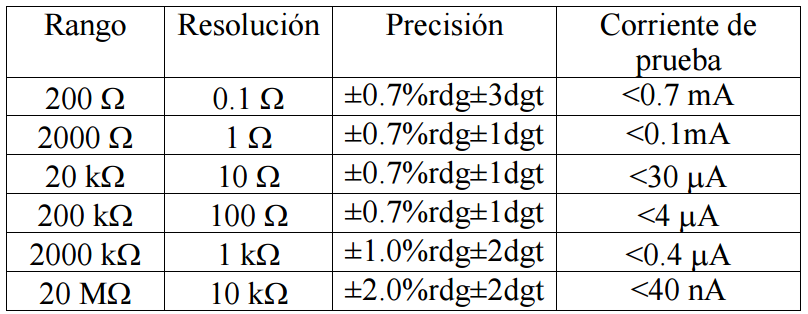
\includegraphics[scale=0.30]{tabla_nominal_resistencias}
\caption{Especificaciones de resistencias}
\end{figure}

Medimos las tres resistencias con el tester, y evaluamos su error según la tabla:
\begin{table}[ht]
\begin{adjustbox}{max width=\columnwidth}

\begin{tabular}{|l | c  c  c | c  c  r |}
\hline
&&Valor Nominal&&&Valor Tester& \\ \hline
Código de colores           &Valor $(k \Omega)$ &$\Delta R (k\Omega)$       &Medición Total $(k \Omega)$ &Valor $(k \Omega)$   &$\Delta R (k \Omega)$  &Medición total $(k \Omega)$ \\ \hline
Verde-Azul-Rojo-Dorado      &5.60                        &0.05                       &$5.60 \pm 0.05$ &5.55                                   &0.05                   &$5.55 \pm 0.05$ \\
Verde-Azul-Rojo-Dorado      &5.60                        &0.05                       &$5.60 \pm 0.05$ &5.51                                   &0.05                   &$5.51 \pm 0.05$ \\ 
Verde-Azul-Amarillo-Dorado  &560                        &4                          &$560 \pm 4$    &555                                    &4                      &$555 \pm 4$ \\
Verde-Azul-Amarillo-Dorado  &560                        &4                          &$560 \pm 4$    &556                                    &4                      &$556 \pm 4$ \\
Verde-Azul-Verde-Dorado     &5600                       &200                        &$5600 \pm 200$ &5380                                   &200                    &5380  $\pm$ 200 \\
Verde-Azul-Verde-Dorado     &5600                       &200                        &$5600 \pm 200$ &5380                                   &200                    &5380  $\pm$ 200 \\ \hline
\end{tabular}

\end{adjustbox}
\caption{Mediciones de resistencias}
\end{table}

Las mediciones con tester resultaron bastante aproximadas 
con respecto al valor nominal. Para la tercera resistencia 
el valor nominal difiere más con respecto al valor medido, 
esto puede ser atribuido a varias causas, por ejemplo al mal
estado de la resistencia, pero aun así es un valor 
relativamente cercano.

\subsubsection{¿Cual de las incertezas influye mas en la calidad de la medida? ¿El porcentual o el relativo a los digitos que indica el tester?}

La incerteza que influye más en la calidad de la medida es la relativa ya que ofrece mas cifras significativas que el error porcentual, el cual se hace sobre el error relativo previamente aproximado dependiendo del número anterior (si es 2,5558 y me pide que tenga 3 cifras significativas quedaría 2,56)

El error porcentual según el enunciado debe tener solo una cifra significativa, hace que sea mas preciso el error porcentual.

\subsection{Mediciones de tensión con un tester}

Armamos el circuito que se indica en la siguiente figura con distintos valores para el set de resistencias.

\begin{figure}[H]
\centering
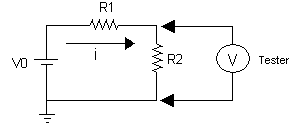
\includegraphics[scale=0.6]{ParteC.png}
\caption{Circuito construido}
\label{fig:1}
\end{figure}

Medimos las tensiones sobre la resistencia $R_2$ y sobre la fuente con el tester y registramos sus valores.
Para cada uno de los circuitos, comparamos los valores experimentales con los teóricos obtenidos en el Problema 5.

\begin{table}[H]
\centering
\begin{tabular}{|c|c|c|c|c|c|}
\hline
\multicolumn{3}{|c|}{Teóricos}&\multicolumn{2}{|c|}{Experimentales}\\\hline
$R_2$ (Ohm) & $\Delta$V (V) & $\Delta$V$R_i$ (V) & $\Delta$V (V) & $\Delta$V$R_2$ (V)\\\hline
5600        & 10            & 4,99               & 10,1          & 4,98\\\hline
560000      & 10            & 4,86               & 9,91          & 4,79\\\hline
5600000     & 10            & 3,9                & 9,94          & 3,96\\\hline
\end{tabular}
\end{table}

El error relativo porcentual entre los valores experimentales y teóricos no supera el 1,5\%

Con respecto a la pregunta presentada en la guía, la segunda ley de Kirchoff dice que, en una malla, la suma de todas las caídas de tensión es igual a la 
tensión total suministrada. De forma equivalente, la suma algebraica de las diferencias de potencial eléctrico en una malla es igual a cero. Esta ley 
siempre se cumple, sin importar que componentes electrónicos estén presentes, la ganancia o pérdida de la energía dada por el campo potencial debe ser cero cuando una carga completa una malla. Sin embargo, según los datos experimentales, la ley de Kirchoff no se cumple, $\Delta V \neq \Delta VR_1 + \Delta VR_2 $. Y podemos apreciar que esta desigualdad es más pronunciada cuando las resistencias del circuito se acercan al valor de la resistencia del votímetro. Un voltímetro ideal tiene una resistencia interna que tiende a infinito, de esta forma, al usarlo, la ley de Kirchoff se cumple porque no hay corriente que vuelva al circuito una vez que pasa por este instrumento. Como no tenemos voltímetros ideales, debemos procurar que los que usemos tengan una resistecia interna considerablemente mayor a las resistencias $R_i$ que se encuentren en el circuito con el que se trabaja.

\subsection{Curvas tensión-corriente de una lamparita}
Para comenzar la experiencia, armamos un circuito cerrado por el cual se conecta una lamparita a la fuente. Comenzamos con corriente y voltaje nulo. Luego, vamos subiendo el valor del voltaje, aproximadamente de a 0,5V, hasta llegar a 12V. Para cada uno de estos valores, registramos el valor de la corriente que le corresponde, y con estos datos calculamos la potencia y resistencia en ese punto.
En la tabla que se encuentra a continuación encontramos los valores de la experiencia. El voltaje está expresado en Volt, la corriente en Ampere; la potencia, calculada como corriente*voltaje, se expresa en Watt y la resistencia, resultado de dividir la potencia por el cuadrado de la corriente, tiene unidad Ohm.

\begin{table}[H]
\begin{adjustbox}{max width= \columnwidth}
\begin{tabular}{|c|c|c|c|c|c|c|}
\hline
\begin{tabular}[c]{@{}c@{}}Voltaje\\   (V)\end{tabular} & Corriente (A) & P = V*i & R=P/i\textasciicircum 2 & \begin{tabular}[c]{@{}c@{}}Con terminales\\   invertidos (A)\end{tabular} & P = V*i & R=P/i\textasciicircum 2 \\ \hline
1                                                       & 0,35          & 0,35    & 2,86                    & 0,4                                                                       & 0,4     & 2,50                    \\ \hline
2                                                       & 0,4           & 0,8     & 5,00                    & 0,45                                                                      & 0,9     & 4,44                    \\ \hline
3                                                       & 0,5           & 1,5     & 6,00                    & 0,5                                                                       & 1,5     & 6,00                    \\ \hline
4                                                       & 0,6           & 2,4     & 6,67                    & 0,6                                                                       & 2,4     & 6,67                    \\ \hline
5                                                       & 0,65          & 3,25    & 7,69                    & 0,65                                                                      & 3,25    & 7,69                    \\ \hline
6                                                       & 0,75          & 4,5     & 8,00                    & 0,7                                                                       & 4,2     & 8,57                    \\ \hline
7                                                       & 0,8           & 5,6     & 8,75                    & 0,85                                                                      & 5,95    & 8,24                    \\ \hline
8                                                       & 0,85          & 6,8     & 9,41                    & 0,9                                                                       & 7,2     & 8,89                    \\ \hline
9                                                       & 0,9           & 8,1     & 10,00                   & 0,9                                                                       & 8,1     & 10,00                   \\ \hline
10                                                      & 0,95          & 9,5     & 10,53                   & 0,95                                                                      & 9,5     & 10,53                   \\ \hline
11                                                      & 1             & 11      & 11,00                   & 1                                                                         & 11      & 11,00                   \\ \hline
12                                                      & 1             & 12      & 12,00                   & 1                                                                         & 12      & 12,00                   \\ \hline
\end{tabular}
\end{adjustbox}
\end{table}


\subsection{Puente de Wheatstone }

Se armó el circuito correspondiente a la experiencia siguiendo el esquema de la figura, teniendo en nuestro caso:

\begin{figure}[ht]
\centering
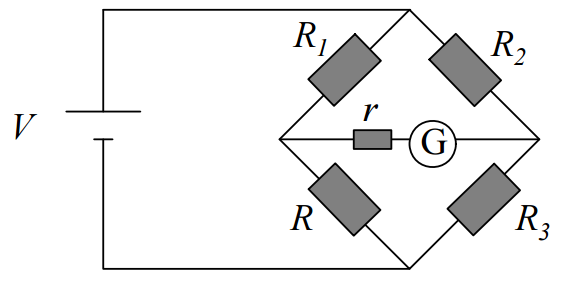
\includegraphics[scale=0.5]{puente_wheatstone}
\caption{Esquema del Puente de Wheatstone}
\end{figure}

\begin{table}[ht]
\centering
\begin{tabular}{|l|c|r|}
\hline
Símbolo &Dispositivo &Valor $\Omega$ \\ \hline
V &Fuente & 6V constante \\
$R_1$ &Resistencia 1 (fija) &(38,8 $\pm$ 0,6) \\
$R_2$ &Resistencia 2 (fija) &(20,8 $\pm$ 0,4) \\
$R_3$ &Resistencia 3 (medido) &(420 $\pm$ 2) \\
$R_v$ &Resistencia (variable) &(227 $\pm$ 2) \\
r &Resistencia de protección &- \\
G &Galvanómetro &- \\ \hline
\end{tabular}

\caption{Referencias  del Puente de Wheatstone}
\end{table}

Para hallar el valor de la resistencia variable, se la varia hasta que la corriente en el galvanómetro sea 0, en ese momento se encuentra en equilibrio. Ese sera el valor que utilizaremos en los cálculos. En nuestro caso la resistencia variable fue de $227 \Omega$
    
Una vez que tenemos el sistema armado, conectamos la fuente y llevamos el puente al equilibrio. Luego cortocircuitamos el sistema colocando una clavija metálica a la resistencia de protección, entonces, para restablecer el equilibrio (i=0 en la rama del galvanómetro)
ajustamos el valor de $R_v$ hasta alcanzar:
$R_v = 227\Omega$

Aplicando la ecuación de equilibrio:

\begin{equation}
R_1 R_v = R_3 R_2
\end{equation}
\begin{align*}
38,8\Omega 227\Omega = R_3 28,8\Omega \\
R_3 = 423,44 \Omega \\
\end{align*}

Y su error asociado por propagación:
\begin{equation}
E_{R3} = \left| \frac{R_v}{R_2} \right| E_{R_1} + 
\left| \frac{-R_1 R_v}{R_{2}^2}\right| E_{R_2} + \left| \frac{R_1}{R_2} \right| E_{R_v}
\end{equation}

\begin{align*}
E_3 = 18,42 \Omega
\end{align*} 

Luego, $R_3 = (420 \pm 20)\Omega$\\



Las fuentes de incerteza de la resistencia incógnita derivan de las incertezas de las otras tres resistencias, que dependen principalmente de la lectura de datos desde el multímetro, como también de la incerteza absoluta propia del aparato para los rangos en los que se están realizando las mediciones.\\
En el caso de las resistencias conocidas, se conoce exactamente su valor. Mediante la aplicación de Kirchhoff y de la condición de equilibrio del puente, podemos anticipar analíticamente el valor de R3. En este caso, se obtuvo un valor mayor al medido a partir de la medición directa con el multímetro. El error pudo haber surgido por:

\begin{itemize}
    \item El grado de exactitud de las resistencias que constituyen el puente.
    \item La agudeza de la visión del observador.
    \item Las uniones entre las resistencias.
\end{itemize}

La ventaja de la utilización del Puente de Wheatstone es que la relación entre las resistencias es siempre la misma cuando no pasa corriente por el galvanómetro con independencia del valor de la corriente.

La operación se reduce a variar las resistencias conocidas, hasta obtener un estado de equilibrio del puente.
\section{Resultados}

\subsection{Curvas tensión-corriente de una lamparita}
Respondiendo a la pregunta presente en el enunciado, que 
nos consulta acerca de si 'es usual que las lámparas 
incandescentes se `quemen' al encenderlas', la respuesta es sí. Al momento de conectar la lámpara, puede ser que la 
corriente sea mayor a la que soporta, por la variación en 
las líneas de tensión. Si pasa esto, se rompe la 
resistencia de la lamparita y se quema. Por este motivo, 
las líneas de corriente se manejan con valores un poco 
menores a los indicados, para así evitar inconvenientes por un valor mayor al supuesto.\\


Utilizando los valores obtenidos de la experiencia,presentes en el cuadro de la sección 'Desarrollo 4.3' y en la tabla a continuación, podemos establecer relación entre el voltaje y la corriente.

\begin{table}[h]
\centering
\begin{tabular}{|c|c|c|cccc}
\cline{1-3}
\textit{\begin{tabular}[c]{@{}c@{}}Voltaje\\   (V)\end{tabular}} & \textit{Corriente (A)} & \textit{\begin{tabular}[c]{@{}c@{}}Corriente con\\   terminales invertidos (A)\end{tabular}} &  &  &  &  \\ \cline{1-3}
1                                                                & 0,35                   & 0,4                                                                                          &  &  &  &  \\ \cline{1-3}
2                                                                & 0,4                    & 0,45                                                                                         &  &  &  &  \\ \cline{1-3}
3                                                                & 0,5                    & 0,5                                                                                          &  &  &  &  \\ \cline{1-3}
4                                                                & 0,6                    & 0,6                                                                                          &  &  &  &  \\ \cline{1-3}
5                                                                & 0,65                   & 0,65                                                                                         &  &  &  &  \\ \cline{1-3}
6                                                                & 0,75                   & 0,7                                                                                          &  &  &  &  \\ \cline{1-3}
7                                                                & 0,8                    & 0,85                                                                                         &  &  &  &  \\ \cline{1-3}
8                                                                & 0,85                   & 0,9                                                                                          &  &  &  &  \\ \cline{1-3}
9                                                                & 0,9                    & 0,9                                                                                          &  &  &  &  \\ \cline{1-3}
10                                                               & 0,95                   & 0,95                                                                                         &  &  &  &  \\ \cline{1-3}
11                                                               & 1                      & 1                                                                                            &  &  &  &  \\ \cline{1-3}
12                                                               & 1                      & 1                                                                                            &  &  &  &  \\ \cline{1-3}
\end{tabular}
\end{table}

Con estos valores realizamos los gráficos que se encuentran a continuación, que representan la relación Voltaje vs Corriente a lo largo de la experiencia, para el caso de terminales "normales" y terminales invertidas. Podemos ver que la diferencia sobre el final del experimento es nula, mientras que durante la etapa media es cuando observamos desigualdades, aunque sean mínimas.

\begin{figure}[H]
\centering
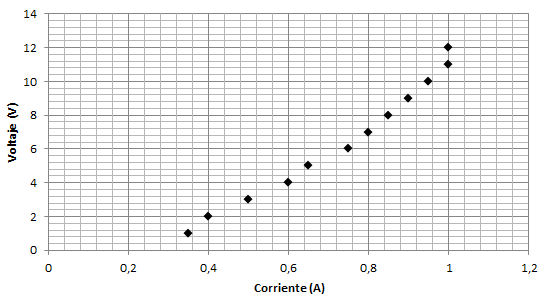
\includegraphics[scale=0.7]{lamparitaTerminalsComunes.png}
\caption{Voltaje en función de la corriente}
\end{figure}

\begin{figure}[H]
\centering
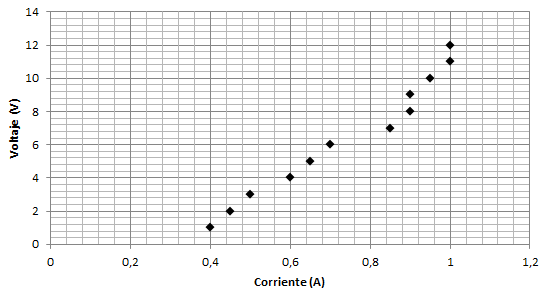
\includegraphics[scale=0.7]{lamparitaTerminalesInvertidos.png}
\caption{Voltaje en función de la corriente para terminales invertidos}
\end{figure}

Además, con los datos de esa misma sección del trabajo (Desarrollo 4.3), podemos estimar la temperatura del filamento de la lámpara en los puntos medidos. Si tenemos en cuenta que la primer columna de la tabla presente en el enunciado refiere a la relación entre la resistividad a cierta temperatura y la misma a 300K, si dividimos cada una de las resistividades medidas por aquella a 300K, obtenemos un valor que se correspondería a la primer columna. Así, teniendo en cuenta entre qué valores de la tabla se encuentra cada uno de los que obtuvimos dividiendo, estimamos la temperatura de la lamparita en cada punto.
También, es posible calcular el coeficiente que representa la variación de la resistividad con la temperatura (To=298K, temperatura ambiente). Se calcula con la fórmula:
\begin{figure}[H]
\centering
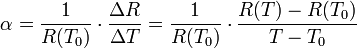
\includegraphics[scale=0.5]{alpha.png}
\end{figure}

Creamos el siguiente cuadro, donde se indica la temperatura 'referencia' en Kelvin y grados centígrados para cada punto y el valor del coeficiente en cada punto.


\begin{table}[H]
\centering
%%%%%%%%%%%%%%%%%%%%%%%%%%%%%%%%%%%%%%%%%%%%%%%%%%%%%%%%%%%%%%%%%%%%%%
%%                                                                  %%
%%  This is a LaTeX2e table fragment exported from Gnumeric.        %%
%%                                                                  %%
%%%%%%%%%%%%%%%%%%%%%%%%%%%%%%%%%%%%%%%%%%%%%%%%%%%%%%%%%%%%%%%%%%%%%%
\begin{tabular}{|l|c|c|c|r|c|}
\hline
Punto	&R	&$R/R_300$	&T(K)	&T(C)  &Coeficiente \\\hline
1	&2,86	&0,51	&$<$ 300	&$<$27  &-0,247\\
2	&5,00	&0,88	&$<$ 300	&$<$27  &-0,058\\
3	&6,00	&1,06	&$\geq$300	&$\geq$27   &0,031\\
4	&6,67	&1,18	&$>$300	&$>$27  &0,090\\
5	&7,69	&1,36	&$\leq$400	&$\leq$127  &0,004\\
6	&8,00	&1,42	&$\approx$400	&$\approx$127   &0,004\\
7	&8,75	&1,55	&$\geq$400	&$\geq$127  &0,005\\
8	&9,41	&1,67	&$\geq$400	&$\geq$127  &0,007\\
9	&10,00	&1,77	&$<$500	&$<$227 &0,004\\
10	&10,53	&1,86	&$\approx$500	&$\approx$227   &0,004\\
11	&11,00	&1,95	&$\geq$500	&$\geq$227  &0,005\\
12	&12,00	&2,12	&$>$500	&$>$227 &0,006\\ \hline
\end{tabular}
\caption{Temperaturas en cada punto}
\end{table}

Con la información del cuadro que se encuentra antes, elaboramos un gráfico donde se representa la relación entre la resistencia en cada punto y el coeficiente en él:

\begin{figure}[H]
\centering
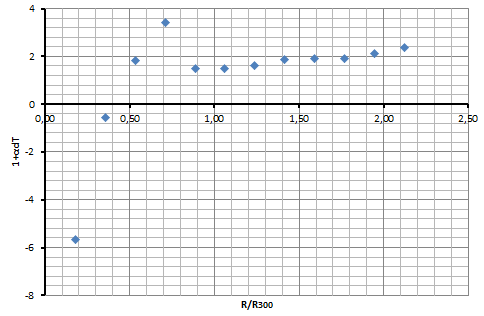
\includegraphics[scale=0.8]{variacionalpha.png}
\end{figure}


\section{Conclusiones}
\begin{itemize}
    \item En cuanto a la primera experiencia, la de las mediciones de las resistencias, se puede remarcar las diferencias entre el valor nominal y el medido con el tester. Esta diferencia es más marcada a medida que los valores de dichos elementos aumentan, concordando con las precisiones que se especifican para cada una. Una causa posible de este error, no mencionada en la parte de desarrollo, es el contacto de los dedos con el tester y las resistencias, actuando nosotros como una.
    \item Podemos destacar el bajo error relativo obtenido en la segunda experiencia, reafirmando de forma práctica la validez de las leyes de Kirchoff y su correlación con la realidad. Si comparamos con el caso anterior, teniendo en cuenta que el instrumento que utilizamos para medir es el mismo, se puede corroborar la teoría de que el error generado era por agregar un elemento extra (nosotros) al circuito, en este caso, los elementos circuitales no tuvieron contacto con nuestro cuerpo.
	\item A medida que avanzamos en la experiencia de la lamparita, nos dimos cuenta que al subir el voltaje,  la subida de la corriente no se desarrolla en forma lineal. Además, el aumento se da solo hasta 1A, ya que para poder llegar a obtener una corriente mayor debíamos llevar la conexión a un potencial más grande que el que resiste la lamparita. Al invertir los terminales, obtuvimos valores similares a los de la primer medición, e incluso en algunos puntos obtuvimos exactamente el mismo valor. Esto nos llamó la atención, ya que anteriormente y de forma errónea creíamos que la experiencia iba a variar de un caso al otro.
    \item Otra observación que se puede mencionar de la práctica con la lamparita, es que la resistencia en frío difiere de la que presenta la misma en funcionamiento. Esto concuerda con la teoría de que la resistencia varía en función de la temperatura.
    \item Acerca del puente de Wheatstone, podemos comentar que a pesar de ser un método sencillo y rápido de aplicar, tiene como punto en contra las incertezas que acarrea (pudiendo observar esto de forma práctica). Al depender un sólo valor de otros tres, el error final termina siendo mucho mayor que para las otras experiencias. Entonces, a pesar de que las incertezas tienen el mismo origen que en los casos anteriores, para esta experiencia resultan mucho más determinantes.
    \item Por último, con respecto a la experiencia referida al fusible, se puede destacar que el mismo no se quemó al llegar a la corrientes máxima "marcada" sino en un valor mayor. 


\end{itemize}
\end{document}